\documentclass[11pt]{article}
\usepackage[margin=1.1in]{geometry}
\usepackage{amsmath,amssymb,amsthm}
\usepackage{booktabs}
\usepackage{array}
\usepackage[protrusion=true,expansion=false]{microtype}
\usepackage{xcolor}
\usepackage{enumitem}
\usepackage{titlesec}
\usepackage{tikz}
\usepackage{float}
\usepackage[normalem]{ulem}
\usetikzlibrary{arrows.meta,positioning,fit,shapes.geometric,calc}
\usepackage{listings}
\usepackage{hyperref}
\hypersetup{colorlinks=true, linkcolor=blue!60!black, urlcolor=blue!60!black, citecolor=blue!60!black}

\titleformat{\section}{\large\bfseries}{\thesection.}{0.7em}{}
\titleformat{\subsection}{\normalsize\bfseries}{\thesubsection.}{0.6em}{}

\newcommand{\transcript}{\bigl(A_{1},A_{2},\textrm{PoKs},\textrm{ctxt},T,\sigma'_{A,P},R_{\cdot\cdot},s_{1},s_{2},e_{1},e_{2}\bigr)}

% macros for the dispute-graph section
\newcommand{\op}[1]{\texttt{OP\_#1}}
\newcommand{\push}[1]{\ensuremath{\langle #1\rangle}}
\newcommand{\Pa}{\mathsf{A}}
\newcommand{\Pb}{\mathsf{B}}
\newcommand{\Hub}{\mathsf{H}}
\newcommand{\tsd}{\Delta}
\newcommand{\dl}{\delta}
\newcommand{\dlp}{\delta'}
\lstdefinestyle{script}{
  basicstyle=\ttfamily\small,
  columns=fullflexible,
  keepspaces=true,
  breaklines=true,
  frame=single,
  framerule=0.3pt,
  xleftmargin=1em,
  escapeinside={(*}{*)},
}

\newtheorem{theorem}{Theorem}
\newtheorem{definition}{Definition}
\newtheorem{remark}{Remark}
\newtheorem{lemma}{Lemma}
\newtheorem{observation}{Observation}
\usepackage[skip=0.6\baselineskip, indent=0pt]{parskip}
\title{\textbf{LN-GAP}\\Lightning governed by arbitrary programs}
\author{waxwing}

\date{September 2026 \\ \medskip Version 1.0 (draft)}

\begin{document}
\maketitle

\tableofcontents

\section{Abstract}

We propose, without any consensus change to Bitcoin, offchain bilateral contracts in Bitcoin that depend on arbitrary computation, calling this general paradigm LN-GAP (Lightning Network governed by arbitrary programs). That general idea is not new but we describe here a distinct mechanism to achieve O(1)-transactions to resolve disputed contracts onchain (that is, there is no onchain bisection). The onchain dispute resolution depends on a threshold attestation of the validators to absence of a published entry, and a 1 of $n$ positive signature over the entry in a novel way (we call this an elliptic curve one time signature, or EC-OTS), and in so doing allows the application of the ForceMove paradigm for the offchain game with an independent timeout clock that does not rely on facts about the Bitcoin chain itself (thus not requiring Bitcoin SPV proofs). The advantages of this construction are: publishing of entries requires only 1 of $n$ liveness, contracts are fully denominated in bitcoin and trust-minimised: they rely on the honesty of a majority of the venue members (a committee that can be drawn per contract from a large bonded roster), whose misbehaviour is attributable and who themselves are not required to execute the contract or program, and fraudulent equivocation is provable. Those validators are motivated by both positive fees (paid, in bitcoin, atomically with publication in LN channels) and negatively by timelocked bonds, reputation loss (attributed fraud) and optionally burning bonds to miner fees.

\section{Introduction}

Start from the \textbf{known good} - that Lightning as a payments technology works, and works well. It aids privacy and scalability, if not perfectly addressing both, it addresses them to a large extent, at the cost of extra infrastructure for users and service providers. Once that infrastructure is in place, the \emph{payments} UI/workflow for users is as smooth as it should be\footnote{For those readers who balk at this characterization, note that the author has been paying his utility bills for years, and along with thousands of other payments during that time with near zero payment failures, on self-custodial Lightning, and for practical, not ideological, reasons, far prefers using LN as a payment technology over any existing fiat rail.}.

What's missing? Lightning already provides private, fast and cheap payments. In vague terms, I would argue that all it really misses is ``programmatic extensibility''. Take as an example this goal:

\begin{quote}
The customer wants to pay a storage service provider once per day, in sats, but wants the service provider to prove that they are upholding their agreement (with a response to a challenge for an inclusion proof), and if they fail to do so after a time window, their deposit can be taken.
\end{quote}

This is basically ``\underline{Filecoin without an altcoin}'', although arguably better. See Section~\ref{sec:storage}.

\subsection{The problem of 2-party games on Lightning}

Suppose you want to play a game on Lightning, like chess, for a monetary reward, but don't want to have to trust anyone; the money should move specifically according to the agreed game rules.

I mention chess not because it's a good game to bet on (it isn't!) but because it's a game that's sufficiently complex that expressing it in onchain transactions (most specifically, proving that a move is illegal; proving that a move is legal would be way worse!) gets very expensive and we want to avoid it.

That such games can be played on chain at all, in today's Bitcoin, was described by Poelstra~\cite{poelstrastate}: each player signs the next game state with a one-time (Lamport) signature, which Script can read, and a script checks that successive states are related by the rules, so tic-tac-toe needs 27 pre-signed transactions rather than one per path through the game tree (about 250,000), and the same approach extends in principle to chess. His distinction between ``Small Script'', expressive arithmetic on 32-bit values that cannot see the transaction, and ``Big Script'', which can, through \texttt{OP\_CHECKSIG}, is a useful lens for what follows: the predicates that judge a move here are Small Script over one-time-signed state, and only the payout is Big Script. What that work leaves open is the one-move-per-transaction pace of play on chain, which is the subject of the rest of this section.

One approach to doing this offchain is called ForceMove~\cite{forcemove}. The idea is relatively simple: behave optimistically, and fallback to onchain transactions as the arbiter if your opponent does not follow the rules you agreed to. The reason for its name is that, once on-chain, the opponent is \emph{forced to move} by having a timeout expressed in the blockchain's consensus logic. So in Bitcoin this would mean that the Script controlling the funds has a shape like: 

\[
\texttt{<}\,T_1\,\texttt{>}\ \ \texttt{OP\_CHECKSEQUENCEVERIFY}\ \ \texttt{OP\_DROP}\ \ \texttt{<}\,P_A\,\texttt{>}\ \ \texttt{OP\_CHECKSIG},
\]

where $P_A$ is the key of the counterparty not on-move, i.e. they win by default if their opponent doesn't move.

This seems to be the right general paradigm: if you're forced to move, the game cannot stall, but your 'move' can be of a type constructed to make it easy to prove fraud whenever the move is illegal. (I haven't bothered to note how terminal states are resolved, i.e. win/lose/draw; that's less important and pretty simple, usually).

\subsubsection{ForceMove is not the full solution}

ForceMove is clearly ``correct''; there is no way to have the game be fair without such a timeout clause. So if you lose the ability to publish within a time window, you forfeit the game. Note that this is exactly the same tradeoff that Lightning itself makes for the case of simple payments.

But the problem with ForceMove, which is not exposed in the Lightning payments case, is that the amount of interaction forced on-chain is potentially huge, depending on the game. Consider this scenario:

\begin{itemize}
\item Alice and Bob agree to play chess offchain, set up a contract in a Lightning channel (details deferred till later)
\item Alice makes move 1 as a message offchain, both sides cosign and state is updated; it's Bob's move.
\item Bob stalls, does not send his move
\item Alice is forced to resolve onchain: sends the state in a transaction, the output has a timeout forcing Bob to respond
\item Bob \emph{does} respond, with a valid move \ldots
\end{itemize}

\ldots now Alice is stuck playing the game onchain; a chess game can easily take 50-100 moves by both sides. If Bob is adversarial he will know that Alice will not want either the transaction cost or especially the delay implicit in doing all of those moves onchain (she intended to play offchain, which can be near immediate), so he could bribe her. This would be much more relevant if the game is really financially motivated (\$ 1000 bet), and in a case where we are at move 30 and Bob knows for sure he's losing; instead of resigning he says to Alice ``here, I'm generous, take \$ 800 and I'll take \$ 200, otherwise, we're going to chain''.

The point is not that that scenario is particularly realistic, the point is that \textbf{going onchain is a viable threat for an adversary}, in general, and that's why I say ``ForceMove is not the full solution''.

\subsubsection{Can we do ForceMove offchain?}

The next natural step. If we want to enforce a timeout clause like the above, but \emph{offchain}, then clearly putting it into a Bitcoin Script is possible, but that returns us precisely to where we started: ForceMove's forced move is only effected on-chain in the adversarial case; the thing we were trying to avoid.

There's a nuance here worth being precise about:

\begin{itemize}

\item If one side forces on-chain, publishing a dispute transaction, and says ``the other guy didn't follow the rules! here's proof'', with a signed attestation by the counterparty of an illegal move, no problem: the court can adjudicate the dispute.
\item If one side forces on-chain, publishing a dispute transaction, and says ``the other guy didn't send his move'', that's very different. How does the ``court'' (blockchain) know whether the move was sent or not? Clearly that's impossible, so the court has to treat both sides fairly, and insist they play out their moves. \uline{We have reverted to exactly the same problem we had in vanilla ForceMove}.
\end{itemize}

From this reasoning it's clear: to solve the problem of that last case, we need an \uline{objective fact} that the court can assess, not hearsay. That objective fact must take the form ``by the count of some external attestation, the counterparty did not post a move before the deadline''. In the next section we'll examine two different ways to create that external attestation on what we'll henceforth call the ``\textbf{venue}''.

The following diagram (Figure~\ref{fig:highlevel}) shows at a high-level how this logic can be enforced in a single ``contract output'' embedded in a Lightning channel. The most important point is that ``the counterparty did not move before the deadline'' is being attested to by an external venue.

\begin{figure}[H]
\centering
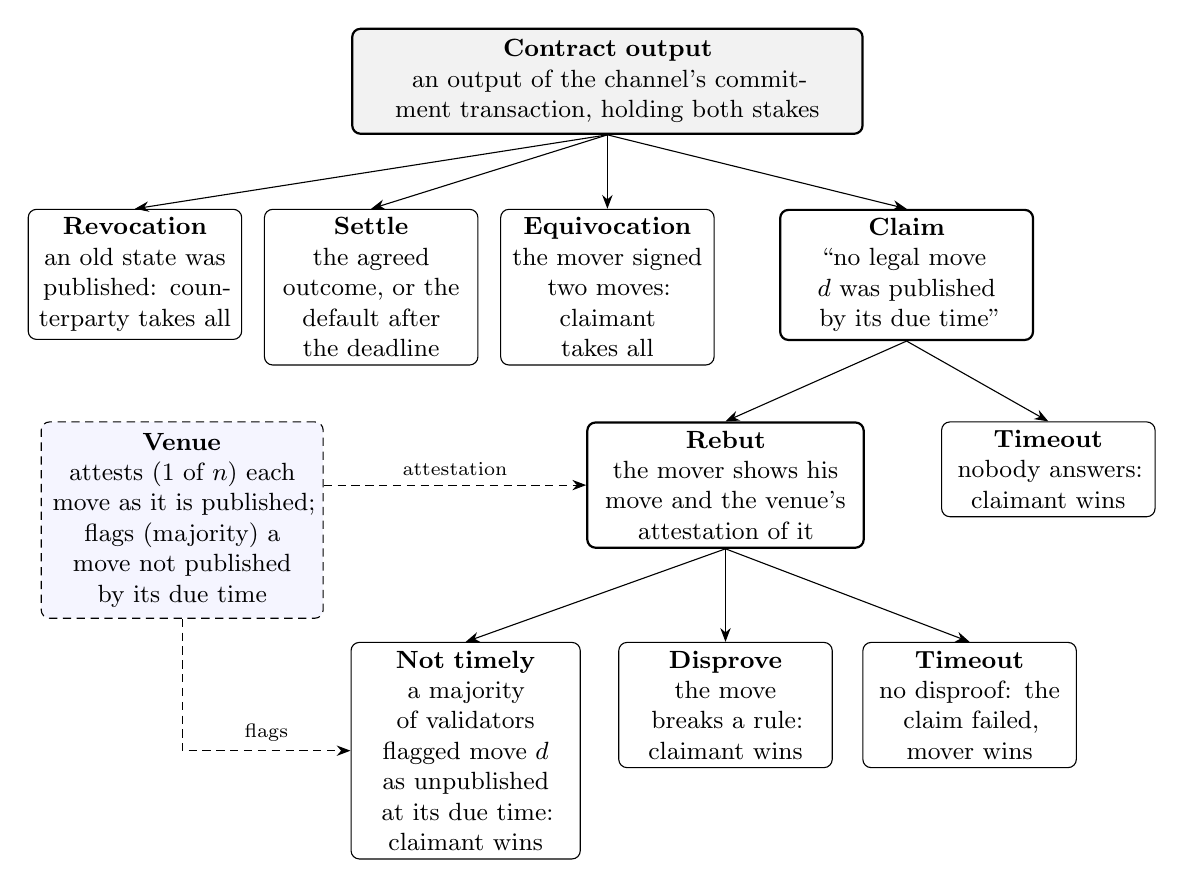
\begin{tikzpicture}[
  font=\small,
  box/.style={draw, rounded corners=3pt, align=center, inner sep=3pt, text width=#1, anchor=north},
  box/.default=25mm,
  cout/.style={draw, thick, fill=black!5, rounded corners=3pt, align=center, inner sep=4pt, anchor=north},
  ven/.style={draw, densely dashed, rounded corners=3pt, align=center, inner sep=4pt, fill=blue!4, anchor=north},
  >={Stealth[length=5pt]},
]
\node[cout, text width=62mm] (C) at (0,0) {\textbf{Contract output}\\ an output of the channel's commitment transaction, holding both stakes};

\node[box] (rev) at (-6,-2.3) {\textbf{Revocation}\\ an old state was published: counterparty takes all};
\node[box] (set) at (-3,-2.3) {\textbf{Settle}\\ the agreed outcome, or the default after the deadline};
\node[box] (eqv) at (0,-2.3) {\textbf{Equivocation}\\ the mover signed two moves: claimant takes all};
\node[box=30mm, thick] (clm) at (3.8,-2.3) {\textbf{Claim}\\ ``no legal move $d$ was published by its due time''};
\foreach \n in {rev,set,eqv,clm} \draw[->] (C.south) -- (\n.north);

\node[box=33mm, thick] (ref) at (1.5,-5.0) {\textbf{Rebut}\\ the mover shows his move and the venue's attestation of it};
\node[box] (to1) at (5.6,-5.0) {\textbf{Timeout}\\ nobody answers: claimant wins};
\draw[->] (clm.south) -- (ref.north);
\draw[->] (clm.south) -- (to1.north);

\node[box=27mm] (nt) at (-1.8,-7.8) {\textbf{Not timely}\\ a majority of validators flagged move $d$ as unpublished at its due time: claimant wins};
\node[box] (dis) at (1.5,-7.8) {\textbf{Disprove}\\ the move breaks a rule: claimant wins};
\node[box] (to2) at (4.6,-7.8) {\textbf{Timeout}\\ no disproof: the claim failed, mover wins};
\foreach \n in {nt,dis,to2} \draw[->] (ref.south) -- (\n.north);

\node[ven, text width=33mm] (V) at (-5.4,-5.0) {\textbf{Venue}\\ attests (1 of $n$) each move as it is published; flags (majority) a move not published by its due time};
\draw[->, densely dashed] (V.east |- ref.west) -- node[above, font=\scriptsize] {attestation} (ref.west);
\draw[->, densely dashed] (V.south) |- node[pos=0.75, above, font=\scriptsize] {flags} (nt.west);
\end{tikzpicture}
\caption{The dispute logic of one contract output, at a high level. Only
the claim and its answers involve the venue: a claim of absence is
answered by the venue's attestation that the move was published, and
that answer is in turn answered either by the game's rules (the move was
illegal) or by the venue again (the move was published too late). Every
branch that pays someone is a Bitcoin transaction prepared in advance;
the arrows are spending conditions, not messages.}
\label{fig:highlevel}
\end{figure}


\subsection{Building the venue - proof of work?}

We defer detailed arguments as to how a proof-of-work consensus system \emph{could} be used for such an ``attestation venue'', and why we ultimately prefer what we broadly call a ``bonded validator quorum'', to the long version of this paper.

\subsubsection{Building the venue - bonded validators}

The alternative is to reach consensus over a quorum, on the list of published values.

It turns out that with careful thought, it's possible to construct a version of this that is both sufficiently efficient to enforce the necessary rules in Script, and also that has the right kind of both positive and negative incentives, purely measured in bitcoin, without inserting a new altcoin.

A naive idea of how to do this hits a snag: Bitcoin Script can read Winternitz signatures in a couple of kilobytes; weighty but OK. It cannot, directly, read Schnorr or BLS signatures on arbitrary messages (the former without CHECKSIGFROMSTACK, the latter .. well that would be a much bigger consensus update!). The latter two can support an aggregated signature; the former (Winternitz, or Lamport) cannot. To assess 66 out of 100 Winternitz signatures in a Bitcoin script seems patently absurd.

Therefore we consider the natural question: can you reproduce the one-time nature of hash-based OTS schemes in an elliptic curve context? We claim that you can, using something we'll call EC-OTS; the details are in Section~\ref{sec:ecots}.

But taking that construction and saying ``we'll have a $\frac{2}{3}$ threshold attest to state updates in an EC-OTS verifiable in Script'' really doesn't give you what you need.

What you need:

\begin{itemize}
\item \textbf{Liveness} : can never be promised, just like in a proof of work chain, but if \emph{any} member of the validator set can enter your publication in a time window, then some approximate ``1 of $n$ liveness'' can be claimed, and this is an acceptable security model.
\item \textbf{A large enough quorum}: Credibility of the above as well as what follows, requires some relatively large, heterogeneous and probably permissionless-entry set of validators. This naturally leads to thinking of FROST-style thresholds, with O(1) publication, but (see next entry) that is not actually viable and so we go with a trick to make thresholds of 50 of 100 be viable. Even figures 10 times higher than that are \emph{theoretically} possible, but in practice we would not go much higher.\footnote{The long version of this paper returns to this: a large, dynamic set need not be verified in Script at all, if its role is to make a small, Script-legible committee accountable.}
\item \textbf{Fraud is attributable}: this is the reason why a naive FROST-style threshold is unworkable: by its nature, such a threshold signature cannot reveal which members of the validator set committed the fraud. And punishing the entire set of such members when only a threshold have committed the fraud, is unacceptable. To make fraud attribution feasible we use what we call a ``one-bit signature'':  $t$ of $n$ OP\_CHECKSIGADD operations can prove that a binary true/false was attested to. More on that in a moment.
\item \textbf{Positive incentives in bitcoin}: this is possible in a more general ``sidechain'' model (pay fees to move around coins on the sidechain), but this is not a sidechain, nor any kind of blockchain: the only consensus maintained is ``did this event get published?''; the semantics of the publications are none of its business. Here we \emph{can} have validators post bonds on bitcoin\footnote{though, as we shall see, there are strong arguments to also use public entities with reputations} (timelocked coins) and receive fees for their publication efforts, atomically with those publications, over Lightning channels, using adaptors. This incentivizes honest participation and disincentivizes fraud or dishonesty.
\end{itemize}

You may be wondering why we insist on \emph{attributable} fraud. Without attribution, users of the venue cannot discern which members they do not want to use in future, if something fraudulent is published. With attribution, a member caught contradicting itself is ejected: it loses its future fees while its bonded coins (coins locked to a CLTV output) sit out their timelock, or its reputation is burned. It's possible to go further, as an option: equivocation evidence can be made to unlock the bonded coins to anyone, but without covenants this is not a simple burn, it is a miner fee-race burn: since the evidence is public, any miner can include its own spend paying the whole bond as fee, so the money game-theoretically ends up with the miner of the first eligible block, and the cheater recovers it only by mining that block itself. We do not include this in the architecture described, but it is a possible additional feature.

\section{EC-OTS: one-time signatures on curve points}
\label{sec:ecots}

Since the introduction of BitVM ideas, we know the paradigm: in the absence of \op{CHECKSIGFROMSTACK}, our best way of dumping a message onto the stack with proof that it was attested by a key owner, is to construct a Lamport/Winternitz signature out of hashes, and the signing event consists of revealing preimages for digit chunks or bits, in the witness of a spending transaction.

This author's original idea was started with the hypothetical of ``can the venue threshold attest using FROST, in Script?'' and wondering how that attestation might make it onto the stack. Though that application of the idea turns out to be bogus, a related idea is very useful: transaction fees for attestations become atomic once the signature is EC-based instead of hash based.

Basically, EC-OTS turns ``knows the discrete log of these points'' into ``attests this value''.

\paragraph{The table.} The venue has a key $X = xG$. For each move of each contract it publishes in advance, for every digit $j$ of the move's head\footnote{We use ``head'' to mean the chunk of data the mover posts; it is not only a move, but also the game or contract state, basically.} (a nibble, $96$ of them for a $48$ byte head) and every value $v \in \{0,\dots,15\}$, an \emph{anticipation point}
\[
A_{j,v} = R_{j,v} + e_{j,v}X, \qquad R_{j,v} = r_{j,v}G, \quad e_{j,v} = H(R_{j,v}, X, \langle\text{contract}, \text{move}, j, v\rangle).
\]

\paragraph{Attesting.} To attest that digit $j$ of the move holds $v$, a member reveals $a_{j,v} = r_{j,v} + e_{j,v}x$. This is a Schnorr signature (with nonce $R_{j,v}$) on the statement ``digit $j$ holds $v$'', whose value is also the discrete log of $A_{j,v}$. Sealing a move means revealing one such scalar per digit.

\paragraph{Reading it in Script.} In a dispute, the mover's Winternitz signature over the head puts the head's digits $v_j$ on the stack; each digit selects $A_{j,v_j}$ from the $16$ points for its position, written into the script as constants, and the spender signs the transaction with $a_{j,v_j}$ as a private key, checked by one \op{CHECKSIG} under $A_{j,v_j}$. The spend is valid only if the venue revealed exactly the scalars for this head. (The $16$ points per position are most of the rebuttal's size in Table~\ref{tab:sizes}.)

\paragraph{One-time.} Revealing two values at the same position is an equivocation, provable by anyone holding both scalars, since each checks against its published point. Each value has its own nonce, so a second value reveals nothing about $x$; with one nonce per position, as in the standard DLC construction, two values would leak the key, which here is shared by every member.

\paragraph{Relatives.} The mechanism is the anticipation points of Discreet Log Contracts~\cite{dlc}, decomposed into digits; the one-time idea is that of Lamport and Winternitz signatures, with curve scalars in place of hash preimages.

\paragraph{Attribution.} Every member holds the same content key, so any member can seal any move (1 of $n$). To say \emph{which} member sealed, each member also has a per-move \emph{proposer point} $P_i = p_iG$ and reveals $p_i$ in its seal; and to flag a move as not published by its due time, a per-move \emph{flag point} $F_i$ whose secret it reveals. These are one-bit versions of the same idea: a point whose secret is revealed, or not. $t$ of $n$ flags are counted in Script with \op{CHECKSIGADD}, each naming its member.


\section{What the venue is not, and a useful prior: DLCs and oracles}
\label{sec:venue}

It might seem that such a ``venue'' is basically a proof of stake blockchain or sidechain. Note that Linus' Stakechains~\cite{coins} pursues that latter idea quite fully, and the reader \emph{will} see some similarities with what's here, but the differences are large, also.

To get the obvious out of the way: it's not a proof of stake \emph{blockchain} as that requires its own token for incentives to validators. Stakechains proposes burn mechanisms for maintaining consensus with slashing, but it is a sidechain, i.e. it creates a separate monetary ledger where side-BTC are exchanged, which means the stakers can be paid in that side asset.

But the deeper disanalogy is that the venue we propose isn't even a proof of publication ledger. It doesn't need to enforce uniqueness of attestations; equivocating attestations are adjudicated within the channel contract. It only has to establish ``X was published in this time window''.

\paragraph{What a venue is also not: a federated sidechain.} This is a natural thought: with a majority attesting, then why bother with complexity? It comes back to a quorum deciding everything. But no: 

\begin{itemize}
\item The federation owns the coins. It can steal all of them, at once, unilaterally (unilaterally with respect to its users, that is). It's crucial to notice that a venue of the type we describe cannot cheat two parties if neither are colluding with a majority of its members.
\item Just another aspect of the above, but a hugely important one: a federation can also freeze any coins it likes. This is practically relevant because of the next bullet point; and note that the Liquid~\cite{liquid} sidechain, for example, only allowed withdrawals to whitelisted addresses. In this scenario freezing is less a theoretical risk and more an inevitability.
\item Federations are comprised of static legal entities, or at least known persons. This prevents the thing that could make them most trustworthy: \emph{permissionless entry}. We achieve this specifically by tying membership to Bitcoin utxos, which means that Sybil is only prevented economically, but allows better trustlessness at scale.
\end{itemize}

The venue's responsibility is isolated: it answers, per move of each contract, the two questions a dispute asks:
\emph{what} was published, and \emph{whether it was published in time}. By the same token, the functionality it provides is not as broad as that of a sidechain or rollup. We will briefly discuss this further in Section~\ref{sec:zk}.

\paragraph{The DLC comparison}. In the terms of Discreet
Log Contracts~\cite{dlc}, the venue \emph{is} a temporary committee of oracles. While each move's \emph{content} is bound to the attestation of one member with anticipation points\footnote{We'll shortly see that this is crucial for the incentives of the system} published in advance, the actual substance of each member's attestation is \underline{the move's timeliness}, not its content, the latter being signed by the mover.

Notice therefore that what is attested --- publication/non-publication within a window --- is of a profoundly different character than a typical oracle attestation (the price of oil in dollars at time $T$):

\begin{quote}
\textbf{The content of the attestation, or the player's ``move'', is a string that can be fed into Script in a form that can allow adjudication of the contract rules; it's not an arbitrary fact that Bitcoin can't read.}
\end{quote}

An oil price posted to a Bitcoin contract proves only that someone claimed that price. Publication is \emph{self-certifying}; a price is not, since nobody can produce evidence of ``the price at noon'', only report it. That leaves only one hole, for our venue: is \emph{when} this ``self-certifying fact'' published, an objective truth?

The answer is ``no'', in the absolute sense, but approaches ``yes'' for longer and longer timescales. Why? Because data can be broadcast --- ``they can't stop the signal, Mal!'' --- and the data here is self-certifying.

Practically, that means if you play games at a cadence of 1 day per move, it is not feasible for members to say ``I said that that move didn't show up in the window because I didn't see it.'' Attribution of fault is still probabilistic for sure, but becomes undeniable in practical terms.

For short term (10 seconds per move), that doesn't apply. Clocks are not perfectly synchronized, so we cannot be sure of fault.

So to summarize the comparison: a price oracle's lie is broadcast and might be immediately visible; it's lying about an external fact. A venue member's lie is only about the time something happened, which is not an external fact. The venue's attestation talks about a much more restricted thing, but is not provable in general; it's only, realistically, provable over longer timescales.

\subsection{Incentives}

\paragraph{Fees.} This is where the use of what we call EC-OTS comes in.

A mover pays the member that seals its move, atomically, with a point-locked payment inside the mover's channel; the typical adaptor trick. The
lock point is $T = C_m + P_{i}$. Think of $C_m$ as the point which represents the player's move (see Section~\ref{sec:ecots}; more details in the long version of the paper), and $P_{i}$ as the point that the member $i$ of the venue pre-selected. All these pre-selected points are sent to the players at the setup of the contract.

The result is that, if the member $i$ ``seals'' the signed move $C_m$, in so doing, it reveals its own secret $p_{i}$, which taken together with the discrete log of $C_m$ is enough for it to claim the fee payment that the mover committed to with an adaptor signature to $T$. This mechanism does not force the member $i$ to actually publish; we discuss these mechanics further in the long version of the paper.

The designated sealer is generally not the payer's channel counterparty,
so the fee must be routed. Since this requires PTLCs, this has implications for the specific Lightning Network in use. While the whole design is possible without fees, the incentives are poor, since without fees, what incentivizes venue members?

\paragraph{Bonds.} Each member can lock bitcoin in a timelocked output on Bitcoin for the duration of its membership. The core function of this utxo is as in Joinmarket fidelity bonds~\cite{fidelity}. It addresses the point that Sybil attacks cannot be prevented directly if identities are unknown, and so the only kind of ``identity'' that exists in Bitcoin itself is at the utxo level. Utxos commit to their role in the venue (or roster of possible members of venue committees). Unfortunately time-value of money cost isn't large unless the amount is large and the time lock is long. We'll see in Section~\ref{sec:security} that there are strong arguments to not \emph{only} use anonymous members.

Because bitcoin doesn't have covenants, one can't constrain that the locked outputs go to, say, burn addresses, under a certain condition. What one can do, as was observed in Stakechains~\cite{coins}, is burn to miner fees by creating an anyone-can-spend output, which is more workable in bitcoin than other systems because colluding sufficiently with miners to actually recoup funds would be nearly completely impractical.

But we have to distinguish two cases:

\begin{itemize}
\item Member \textbf{equivocates} : signs two messages that contradict each other. Even though this can be just ``fault'' (e.g. crash) rather than malicious behavior, as in Lightning, it might make sense to swipe funds here, as earlier mentioned: which in this case means burn to miners.
\item Member attests to something that is publicly obviously false: such as, attesting that a move was not made when it was, at a long timescale. Here the crucial point is that their attestation is public, and the fact that they are lying about is also public. Here the rejection of them is a matter of client choice: those wishing to construct quora for future contracts will not use them, which means they lose all fee revenue in future.
\end{itemize}

The shape of that second item is why two things in the technical design are so important: that it is possible to identify individual members who have attested ``that move is not published in time'' and ``that move is published in time'', and secondly, that there are positive fees to accrue for behaving honestly. With those two elements in place, it's reasonable to argue that the incentives are sufficiently aligned.

\section{Contract outputs and the dispute graph}
\label{sec:graph}

This is a \underline{very abbreviated} version of the description in the long form of the paper; if you want to understand the Script-level mechanics of these contracts, I highly advise reading that version.

Throughout, $\Pa$ and $\Pb$ are the two players ($\Pa$
white, $\Pb$ black); each holds a payment key $P_\Pa$, $P_\Pb$, and every 2-of-2 leaf below is
\[
  \push{P_\Pa}\ \op{CHECKSIG}\ \push{P_\Pb}\ \op{CHECKSIGADD}\ \push{2}\ \op{NUMEQUAL}
\]

Timelocks: $\tsd$ is the channel's \texttt{to\_self\_delay}, $\dl$ the challenge window and $\dlp$ the additional delay on prover-favourable paths; move $d$ is due at $T_d = t_0 + d\ell$ and a depth-$d$ absence claim is admissible once median-time-past has passed $T_d + m$ (an absolute, time-based \op{CLTV}).

In setup, the two parties agree several things: first the committee of members is fixed, who are going to form the venue and ``attest'' as discussed extensively above. Then, they will need to get, from those members, all the per-move keys: keys for ``anticipation points'' used for constructing atomic fees; keys for ``flags'' that let them attest to non-publication. $\Pa$ and $\Pb$ will also need to share a big chunk of similar keys with each other: Winternitz keys for rebuttal and for state.

That whole setup \emph{is} linear in the finite number of moves that the contract or game can take up: worth emphasizing, because it means that our applications must consider only reasonable finite-length games (at least, in this design). The dispute graph (see Figure~\ref{fig:graph}) must be pre-signed for all future moves.

What remains is an augmentation of Lightning: cosigning a commitment transaction which now has a special contract output $C$. Like to\_local, $C$ carries Lightning's revocation leaf, so a revoked state is swept in full (every leaf of $C$ that the broadcaster could use first waits out the channel's \texttt{to\_self\_delay}, so nothing escapes the sweep by spending $C$ early); and $C$ has equivocation leaves that work similarly: if a party signs two different states at the same depth with its Winternitz key, the counterparty takes the whole pot.

A move thus does not require a channel update; though, a fee might; this can be avoided; \underline{see the long version of the paper} for details on this and a lot more about this design.

\begin{figure}[t]
\centering
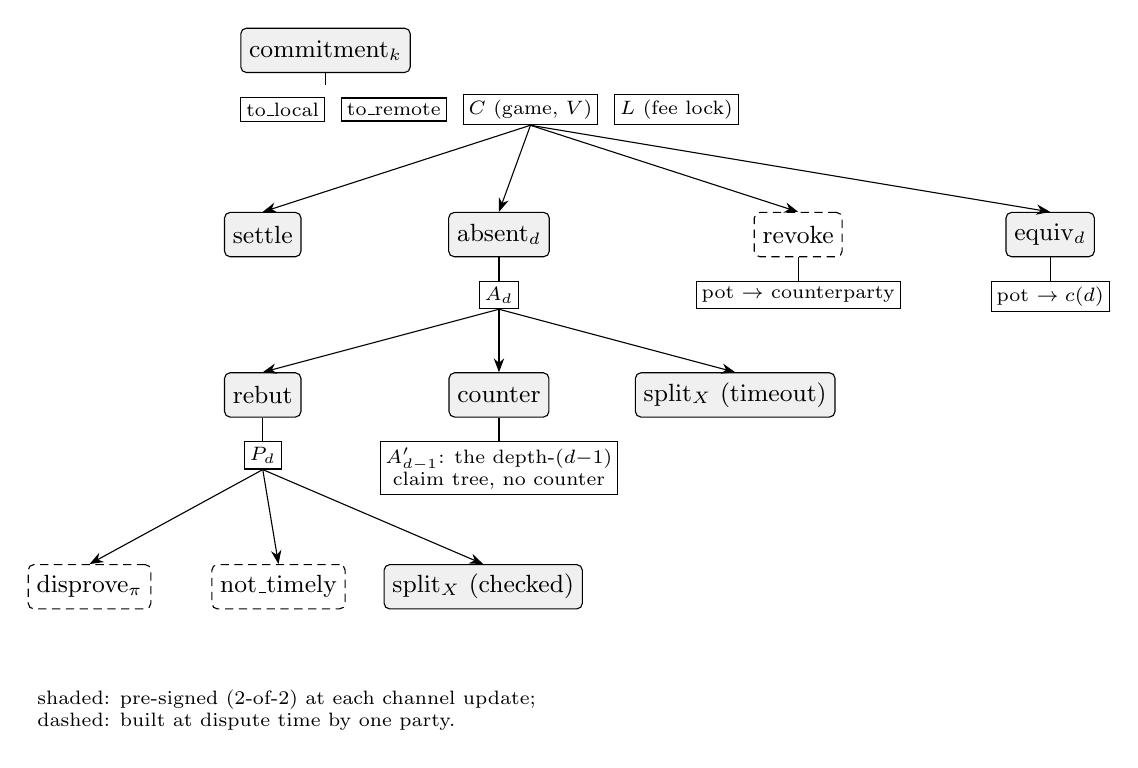
\begin{tikzpicture}[
  font=\small,
  tx/.style={draw, rounded corners=2pt, minimum height=1.6em, inner sep=3pt, align=center},
  pre/.style={tx, fill=black!6},
  run/.style={tx, densely dashed},
  outp/.style={draw, fill=white, inner sep=2pt, font=\scriptsize},
  >={Stealth[length=5pt]},
  every edge/.style={draw, ->},
  node distance=6mm and 9mm,
]
\node[pre] (commit) {commitment$_k$};
\node[outp, below=3mm of commit.south west, anchor=north west] (tl) {to\_local};
\node[outp, right=2mm of tl] (tr) {to\_remote};
\node[outp, right=2mm of tr] (C) {$C$ (game, $V$)};
\node[outp, right=2mm of C] (L) {$L$ (fee lock)};
\draw (commit.south) -- ++(0,-1.5mm);

\node[pre, below=11mm of C, xshift=-34mm] (settle) {settle};
\node[pre, below=11mm of C, xshift=-4mm] (absent) {absent$_d$};
\node[run, below=11mm of C, xshift=34mm] (revoke) {revoke};
\node[pre, below=11mm of C, xshift=66mm] (equiv) {equiv$_d$};
\foreach \n in {settle,absent,revoke,equiv} { \draw (C.south) edge (\n.north); }

\node[outp, below=3mm of absent] (Ad) {$A_d$};
\draw (absent) -- (Ad);
\node[pre, below=8mm of Ad, xshift=-30mm] (rebut) {rebut};
\node[pre, below=8mm of Ad, xshift=0mm] (counter) {counter};
\node[pre, below=8mm of Ad, xshift=30mm] (tsplit) {split$_X$ (timeout)};
\foreach \n in {rebut,counter,tsplit} { \draw (Ad.south) edge (\n.north); }

\node[outp, below=3mm of rebut] (Pd) {$P_d$};
\draw (rebut) -- (Pd);
\node[run, below=12mm of Pd, xshift=-22mm] (disprove) {disprove$_\pi$};
\node[run, below=12mm of Pd, xshift=2mm] (nt) {not\_timely};
\node[pre, below=12mm of Pd, xshift=28mm] (csplit) {split$_X$ (checked)};
\foreach \n in {disprove,nt,csplit} { \draw (Pd.south) edge (\n.north); }

\node[outp, below=3mm of counter, align=center] (Adm) {$A'_{d-1}$: the depth-$(d{-}1)$\\claim tree, no counter};
\draw (counter) -- (Adm);

\node[outp, below=3mm of revoke, font=\scriptsize] (Prev) {pot $\to$ counterparty};
\draw (revoke) -- (Prev);

\node[outp, below=3mm of equiv, font=\scriptsize] (Peq) {pot $\to c(d)$};
\draw (equiv) -- (Peq);


\node[anchor=north west, font=\scriptsize, align=left] at ($(disprove.south west)+(0,-9mm)$)
  {shaded: pre-signed (2-of-2) at each channel update;\\
   dashed: built at dispute time by one party.};
\end{tikzpicture}
\caption{The game output $C$ on one commitment and the transactions
hanging off it, per depth $d$. Every output is a taproot tree; the
edges are its leaves. The claim output $A_d$ races the mover's
rebuttal against the claimant's timeout; the rebuttal output $P_d$
races the claimant's disproves against the mover's self-checking split;
the counter sends the game one depth back. ``revoke'' is Lightning's revocation path; it is also a leaf of to\_local and $L$ (not drawn).}
\label{fig:graph}
\end{figure}

\subsection{Measured sizes, scale limits}
\label{sec:graph:sizes}

Table~\ref{tab:sizes} gives virtual sizes, from the proof of
concept's test suite~\cite{lngapcode}, as confirmed on a regtest
node with real timelocks, for a five-member venue ($n=5$, $t=3$).

\begin{table}[t]
\centering
\small
\begin{tabular}{llr}
\toprule
transaction & who & vB \\
\midrule
commitment (two balances, one contract) & broadcaster & $\approx 240$ \\
\texttt{absent}$_d$ & claimant & $188$ \\
\texttt{split}$_X$ (timeout, off $A_d$) & claimant & $193$--$201$ \\
\texttt{counter} & mover & $178$ \\
\texttt{rebut}, tic-tac-toe, $d \ge 2$ & mover & $20{,}106$ \\
\texttt{rebut}, chess, $d \ge 2$ & mover & $24{,}121$ \\
\texttt{rebut}, chess, $d = 1$ (one head) & mover & $19{,}558$ \\
\texttt{disprove}, chess (one exhibit) & claimant & $\approx 4{,}950$ \\
\texttt{not\_timely} ($3$ of $5$ flags) & claimant & $254$ \\
\texttt{split}$_X$ (checked, off $P_d$) & mover & $\approx 4{,}900$ \\
fee \texttt{claim} & payee & $171$ \\
fee \texttt{timeout} & payer & $147$ \\
\bottomrule
\end{tabular}
\caption{Confirmed virtual sizes. A stall costs the claimant two small
transactions at any depth; the rebuttal is the one large transaction
and is paid by the party that answers a claim, its cost being mostly
the venue readout of the new head ($96$ possession proofs, $16$ points
each, as script constants); the prior head is bound by the claimant's
own signature instead. Changing from a 5 member venue to 50 is likely only to add 1\% to the size of the chess rebut transaction; it's linear but very small in magnitude, and the committee size is not practical above about 100 most likely, and impossible above 999 in the current design.}
\label{tab:sizes}
\end{table}

Note that by far the bulk of the onchain cost is always in the rebut step, as that is the step that dumps the actual contract/game state. Obviously, that will almost never appear, but even when it does we are bounded to at most 4 transactions, hence the O(1) claim of the abstract. But importantly, through use of deposit amounts in-channel, one can ensure that the offender is always the one that pays the additional onchain transaction costs.

An additional important scaling detail: we are sensitive to the requirement to have the venue support large numbers of members: the cost of supporting say 100 members instead of 10 is fairly minimal: one point in the script and one witness element per member. The real limit in the current design is the support of \op{CHECKSIGADD} based multisignature attestation to absence; theoretically capped at 999 but realistically we wouldn't go much above 100 members.

\section{Applications}
\label{sec:apps}

\subsection{Storage contracts: Filecoin without an altcoin}
\label{sec:storage}

We return to the example of the introduction.

In short, you can request probabilistic proof of storage~\cite{jk}~\cite{sw} of some large chunk of data from a provider (think: Merkle proof for a random data chunk). This idea was pursued in the altcoins Sia~\cite{sia} and Filecoin~\cite{filecoin}. Because they base actual \emph{blockchains} on this idea, where rewards are built from these proofs, faults are punished with burn. So arguably this design is bad from two angles: one, a public blockchain isn't scalable and necessitates a new token, and two, punishment isn't directed to the aggrieved party (who lost their data).

In the LN-GAP model, instead, a customer can engage with a service provider in a long-term game of challenge-response.

\paragraph{What is new here:} Paying for proofs of retrievability over
Bitcoin has been proposed before: contingent service payments on
Bitcoin for exactly this~\cite{zkcsp}, recurring variants~\cite{rcpor},
periodic challenge-and-pay over a payment channel~\cite{scrypt}, and
per-download payments with a bond and fraud proof over
Lightning~\cite{bitstream}. All are \emph{pay on success}: if the
provider does not answer, the customer does not pay, and the only
penalty for losing the data is lost future income. No two-party
construction can do better, because silence cannot be adjudicated
between two parties. In LN-GAP, however, with a public clock ``no timely response in epoch
$k$'' is a fact, so the provider's \emph{bond} is forfeited for absence,
not merely its payment withheld, and the whole schedule runs off-chain.

\subsection{Hidden information: blackjack}
\label{sec:blackjack}

A browser-based demo is fully implemented in the proof of concept code.

Since Bitcoin is money, we are interested in resolving dispute about payment, and betting on chess is uninteresting. So if we are talking of games, we're talking of staking and betting in some sense. One naturally thinks therefore of hidden-information games where there may or may not be skill involved, but there is also a random element.

To play a simple card game like Blackjack\footnote{If, like the author, you didn't really know the rules of Blackjack, they are summarized in the long version}, we have to handle a fairly simple state machine over cards and hands, but the hidden information part is different. We start from the known trick of ``combine two parties' randomness, where each is committed upfront so you can't renege''\footnote{Such protocols usually have a fatal flaw: the last mover has full information so can renege if they don't like the outcome; LN-GAP addresses precisely that problem: stalling your move is a loss!}.

Opening a commitment is a problem in Script, because commitments have to be ``hiding'' and that is usually achieved with concatenating a salt. But, there is no \op{CAT}. Instead the value is
encoded in the \emph{length} of a random string, as in the Bitcoin
lottery of Andrychowicz et al.~\cite{smcbitcoin}: commit
$C = \mathrm{SHA256}(s)$ with $|s| = 32 + v$ bytes; to open, reveal $s$,
and the script checks the hash and reads $v$ with \op{SIZE}.

It's a very cool trick, but notice it only allows committing to quite small numbers, so for many applications it won't be useful. Here it works perfectly.

To deal a card, you take such a commitment from both players, open and combine it by simply adding the two numbers mod 13 to deal a card. Now obviously dealing with replacement isn't correct for many card games, but apparently in Blackjack it's normal to use a lot of decks so having the equivalent of an infinite shuffled deck is fine.

\subsection{A sealed-bid auction}
\label{sec:auction}

An outline discussion of this idea is deferred to the long version of this paper.

\section{Zero knowledge verifiers --- towards rollup bridges}
\label{sec:zk}

Remember that in the BitVM1 design we had an algorithm\footnote{I think it may be fairer to attribute the original idea to Arbitrum, however} that later designs optimized out: onchain bisection. In LN-GAP, we can do the challenge-response mechanism offchain, relying on the venue, as usual, to prevent stalling. Thus, even if the program is far too big to be dumped onto the stack in Script, by applying this paradigm we can break its execution into chunks offchain, punish stalling and thus enforce that the single chunk of execution under dispute gets resolved in onchain transactions, if there is a dispute.

A very similar approach is taken in BitVMX~\cite{bitvmx}. There, a Groth16 verifier is bisected, but onchain. That offchain vs onchain distinction is the only delta, hence our proof of concept code shows verification of a ZKP \emph{offchain} by use of our publication venue, but otherwise uses the same machinery taken directly from the BitVMX codebase: the Groth16 verifier checking a shrink-wrapped RISC Zero proof of correct execution of a STARK verifier. So the credit is very much theirs; the claimed value in what we do is specifically in making a tradeoff to prevent a very large number of Bitcoin transactions needing to be published. More details in the long version of the paper, but needless to say this specific ``application'' is really a way of opening up a near infinite number of applications, since the program's (the one whose correct execution is STARK-proved at the base layer) size can be made arbitrarily large. It's only because of this possibility that the ``A'' in LN-GAP can truly be asserted.

While this is currently speculative, one can imagine zk-rollup (see~\cite{lightrollups} for potential designs)  hybrid constructions: correctness of a burn from the rollup can be used in a contract with a liquidity provider: demonstrating that the withdrawal claim is consistent with a published history of state roots. Unlike Ethereum, we cannot have a base layer contract provide this, effective, single use seal for the ``hard'' confirmations or finality, so another mechanism, possibly including the use of the venue, and possibly including \op{RETURN} mechanisms, may be required. 

\section{Security}
\label{sec:security}

The long version of the paper tabulates and analyzes different risks inherent in the design. Here, we'll consider a concrete use case to clarify better what the actual risk profile is, and the interesting ways it's different from other similar systems.

The short version is: the content of the contract rules is defended by cryptography + Bitcoin consensus. The ability to publish your next move in the game/contract is defended by a 1 of $n$ availability argument on the venue. The timeliness of your publication --- did you publish before the deadline --- is defended by a majority consensus on the venue, and reputational or economic costs from attributable mis-attestation.

Compare two cases: a federation, using a threshold multisig, decides whether withdrawals are accepted, versus the LN-GAP model:

\paragraph{Federation majority or threshold:} Can steal (or be hacked of) \underline{all funds} in the rollup immediately (it can ignore the status of ZKPs and just sign the transfer on bitcoin). Can censor withdrawals with a $1 - f$ threshold.
\paragraph{LN-GAP venue majority:} has no ability to steal if neither counterparty cooperates with it. \emph{Can} steal for one bilateral relationship, by colluding with one party against the other. \emph{Cannot} steal all funds at the same time unless the aforementioned collusion happens with every counterparty. Can never censor funds at any threshold $f$, since the funds are never under its control unilaterally.

These distinctions have far reaching implications. Notice that ability to steal is also ability to freeze, so in case of public entities, you inevitably have a big funds freezing risk; this was emphasized already in Section~\ref{sec:venue}. Consider this very concrete scenario:

\paragraph{The Iranian service provider:} Alice and Bob-the-service-provider are in Iran and choose a venue, consisting of majority public American companies. Those American companies are subject to sanctions, but didn't know, at contract setup time, that Alice and Bob operate in Iran. After some steps are executed in the Alice-Bob channel, these companies discover this, and by law are required to stop offering service. They cannot freeze the funds; they never controlled them (which is rather helpful to their lawyers!), and it is illegal to collude with either party. Their refusal to participate \emph{does} cause a problem; if Alice and Bob don't perfectly trust each other (else why are they using a cryptographic contract), they have an unstable situation: they can continue, getting moves sealed by other entities (not the American majority), but a majority ``not-timely'' condition can no longer be triggered, meaning stalling (not playing a move) is not safe to publish a claim against, meaning that: they might have to negotiate a co-spend of the output, rely on a long time delay refund or use some kind of fresh re-negotiation of the contract rules continuation with another venue\footnote{they cannot swap-out members mid-contract: the venue members must be fixed at the start, in LN-GAP. Such a re-negotiation protocol is left as future work, but seems intuitive.}. There are two lessons: this model is much better than having funds confiscated from both parties, and, that it's quite necessary to have permissionless or otherwise non-homogeneous elements of the committee.

Another very important point is public attribution. If members of an LN-GAP venue are known, objectively, to have lied about their attestations, then if they are public entities, they have burnt their reputation. If they are anonymous but bonded, they have forgone at least time value of money (if they can no longer use that bond for collecting venue fees). However whether attribution is public or not, as argued in Section~\ref{sec:venue}, is largely a matter of timescales: it is, for longer timescales.

Finally, there is the question of liveness and censorship resistance; we claim it is in general ``1 of $n$''. But it's related to the practical question: ``Who should the venue members be?''. If we use only some set of, say 15 public companies, as venue members it does have an advantage: they have a lot to lose by publically lying about a contract publication fact as discussed in the previous paragraph (attribution) but it loses the natural censorship resistance: they can simply refuse to publish a move for certain entities. While with purely anonymous venue members, the power of 1 of $n$ really kicks in; but if you relied \emph{exclusively} on anonymous venue members, even ones defended with timelocked bonds, you'd be significantly more open to potential Sybil attacks; remember that the Sybils only have to occupy 51\% of the venue membership, plus collude with your counterparty.

This balance is what suggests a probable optimum configuration: some set of public, well known identities with reputations at stake, along with free permissionless-entry anonymous entities, combined to make the quorum. Both would earn transaction fees.

At least one further measure can expand the attack cost: committees drawn per contract, so that a targeted attack reaches one pot and a broad one needs a share of a large roster. We discuss this next in Section~\ref{sec:accountable}.

Finally, we should note that these security gains are not gotten for free: relying on funds in bilateral contracts obviously limits the kinds of contracts that can be executed, and most significantly, implies holding of collateral within those bilateral contract outputs, so the liquidity story is less desirable, in the general case.

\section{Weakening the majority assumption}
\label{sec:accountable}

The long version of the paper discusses additional improvements to the attributability of fault and the reduction of probability of collusion. Here we just mention the most basic mechanism that is almost inevitable in a real world deployment. First we mention the majority threshold's basic reasoning.

\subsection{The threshold adversary}
\label{sec:threshold}

A majority of the members plus your counterparty can take the pot of any contract, in either
direction. By \emph{false flags}, $t$ members declare an honest mover's
timely move unpublished and \texttt{not\_timely} kills its rebuttal.
By a \emph{late seal with suppressed flags}, one member seals a stalling
mover's move after its due time while $n - t + 1$ members withhold their
flags, so the late rebuttal stands. The majority threshold balances
the two, each needing about half of the members. This resembles a
majority attack on a proof-of-work chain.

\subsection{Committees drawn from a roster}
\label{sec:roster}

Notice, the venue is already per contract in everything but its membership: tables, proposer and flag points, due times and the registry are all keyed by the contract
(Section~\ref{sec:venue}), and nothing ties two contracts' members together.

We propose that each contract's members, its \emph{committee}, be drawn at random from a larger \emph{roster} of bonded members. There is then no single venue but one per contract, each sampled from the same roster. A member's work falls rather than rises: it serves only the contracts it is drawn for, about $n/R$ of them for committees of $n$ from a roster of $R$. The committee's size is limited by Script (its flag points are counted in a leaf); the roster's is not.

The choice of members can be using standard provably fair randomness techniques (block hashes etc. etc.), or by other selection procedures. We refer back to the ``probable optimum configuration'' of Section~\ref{sec:security}.

\section{Related work}
\label{sec:related}

ForceMove~\cite{forcemove} and state channels are the paradigm we
modify; Lightning~\cite{lightning} the base we build on. Single-use seals
and proof of publication are due to Todd~\cite{toddseals}, and
OpenTimestamps~\cite{ots} is their simplest deployment; RGB~\cite{rgb}
builds client-side-validated assets on them, and its companion Prime
design places commitments in a dedicated header chain anchored to
Bitcoin. The bonded, Bitcoin-collateralised validator set with one-time
signatures is Linus's Coins and Stakechains~\cite{coins}; what is new
here is that the venue settles no value and carries no asset, and that
its attestations are read in Bitcoin Script. BitVM~\cite{bitvm} settles
arbitrary computation on Bitcoin by bisection; we avoid on-chain
bisection by giving each game a family of single-step disprove leaves.
BitVMX~\cite{bitvmx} does the same for a RISC-V CPU whose execution
trace is a hash chain, with an $n$-ary search over the trace and a
family of single-step challenges at its end; there the search is played
on chain, as a graph of transactions pre-signed at setup with a relative
timelock on each move, trusting nothing beyond Bitcoin. Our
zero-knowledge application (Section~\ref{sec:zk}) takes its CPU,
emulator, search, step scripts and Groth16 verifier program from the
BitVMX codebase, and differs in where the search is played: on the
venue, with only its final step on chain. ESSPI~\cite{esspi}, from the
same authors, publishes large program inputs on Bitcoin before a
timelocked deadline, the public clock of this paper used once per
dispute rather than once per move.
StackSat-128~\cite{stacksat} is a Script-friendly hash designed for the
proof-of-work alternative. The attestation primitive is that of Discreet
Log Contracts~\cite{dlc}: an oracle publishes anticipation points in
advance and reveals the scalar for the outcome that occurred, and a
contract conditions on it; the venue is a committee of such oracles,
attesting publication and timeliness rather than external events, and
its attestations are read out in Script rather than consumed by adaptor
signatures alone. For storage, see Section~\ref{sec:storage}; for hidden-information games, Section~\ref{sec:blackjack}.

\section{Conclusion}

The TLDR is something like this:

\begin{quote}
Lightning cannot adjudicate silence. If it could, you could, without use of very weighty and advanced cryptography like garbled circuits and similar, resolve disputes over complex (not arbitrarily complex, but complex) contracts (or ``program outputs'') in-channel optimistically, with the fallback to onchain Script adjudication limiting program complexity. You could even push that further with offchain bisection of arbitrarily large programs. But you can do none of this because Lightning cannot adjudicate silence. So you craft, carefully, a consensus mechanism over the one fact of publication or non-publication in a time window by contract counterparties, with incentives both positive and negative to make it as healthy as possible.
\end{quote}

\begin{thebibliography}{99}

\bibitem{lightning} J.~Poon and T.~Dryja. The Bitcoin Lightning Network: Scalable off-chain instant payments, 2016. \url{https://lightning.network/lightning-network-paper.pdf}

\bibitem{poelstrastate} A.~Poelstra. Script state from Lamport signatures. Blockstream blog, 3 July 2024. \url{
https://blog.blockstream.com/script-state-from-lamport-signatures/}

\bibitem{forcemove} T.~Close and A.~Stewart. ForceMove: an $n$-party state channel protocol. Magmo, 2018.

\bibitem{toddseals} P.~Todd. Preventing consensus fraud with commitments and single-use-seals, 2016. \url{https://petertodd.org/2016/commitments-and-single-use-seals}

\bibitem{ots} OpenTimestamps. \url{https://opentimestamps.org}

\bibitem{rgb} RGB Protocol. \url{https://rgb.info}

\bibitem{coins} R.~Linus. Coins: a billion Bitcoin users, 2020; R.~Linus and B.~Tse, Stakechains, CoDecFin 2022.

\bibitem{bitvm} R.~Linus. BitVM: compute anything on Bitcoin, 2023.

\bibitem{bitvmx} S.~D.~Lerner, R.~Amela, S.~Mishra, M.~Jonas and J.~\'Alvarez Cid-Fuentes. BitVMX: a CPU for universal computation on Bitcoin, 2024. \url{https://arxiv.org/abs/2405.06842}

\bibitem{esspi} S.~D.~Lerner, M.~Jonas and A.~Futoransky. ESSPI: ECDSA/Schnorr signed program input for BitVMX, 2025. \url{https://arxiv.org/abs/2503.02772}

\bibitem{fidelity} C.~Belcher. Design for improving JoinMarket's resistance to sybil attacks using fidelity bonds, 2019. \url{https://gist.github.com/chris-belcher/18ea0e6acdb885a2bfbdee43dcd6b5af}; and JoinMarket, \emph{Fidelity bonds} (documentation). \url{https://github.com/JoinMarket-Org/joinmarket-clientserver/blob/master/docs/fidelity-bonds.md}

\bibitem{stacksat} AbdelStark. StackSat-128, 2025. \url{https://github.com/starkware-bitcoin/stacksat128}

\bibitem{jk} A.~Juels and B.~S.~Kaliski. PORs: proofs of retrievability for large files. ACM CCS 2007.

\bibitem{sw} H.~Shacham and B.~Waters. Compact proofs of retrievability. ASIACRYPT 2008.

\bibitem{zkcsp} M.~Campanelli, R.~Gennaro, S.~Goldfeder and L.~Nizzardo. Zero-knowledge contingent payments revisited: attacks and payments for services. ACM CCS 2017. \url{https://eprint.iacr.org/2017/566}

\bibitem{rcpor} A.~Abadi, S.~J.~Murdoch and T.~Zacharias. Recurring contingent payment for proofs of retrievability, 2021. \url{https://eprint.iacr.org/2021/1145}

\bibitem{scrypt} sCrypt. Pay for storage using proof of retrievability on Bitcoin. \url{https://scryptplatform.medium.com/pay-for-storage-using-proof-of-retrievability-on-bitcoin-d5f2df009e1}

\bibitem{lngapcode} LN-GAP proof-of-concept code. \url{https://github.com/AdamISZ/ln-gap}

\bibitem{liquid} J.~Nick, A.~Poelstra and G.~Sanders. Liquid: a Bitcoin sidechain, 2020. \url{https://blockstream.com/assets/downloads/pdf/liquid-whitepaper.pdf}

\bibitem{dlc} T.~Dryja. Discreet Log Contracts, 2017. \url{https://adiabat.github.io/dlc.pdf}

\bibitem{sia} Sia Foundation. About providing storage on Sia. \url{https://docs.sia.tech/provide-storage/about-hosting-on-sia}

\bibitem{filecoin} Filecoin documentation: slashing. \url{https://docs.filecoin.io/storage-providers/filecoin-economics/slashing}; storage deal flow, \url{https://spec.filecoin.io/systems/filecoin_markets/onchain_storage_market/storage_deal_flow/}

\bibitem{lightrollups} J.~Light. Validity rollups on Bitcoin, 2022. \url{https://bitcoinrollups.org}; announced on the bitcoin-dev mailing list, October 2022.

\bibitem{smcbitcoin} M.~Andrychowicz, S.~Dziembowski, D.~Malinowski and {\L}.~Mazurek. Secure multiparty computations on Bitcoin. IEEE Symposium on Security and Privacy, 2014. \url{https://eprint.iacr.org/2013/784}

\bibitem{bitstream} R.~Linus. BitStream: decentralized file hosting incentivised via Bitcoin payments, 2023. \url{https://robinlinus.com/bitstream.pdf}

\end{thebibliography}

\end{document}
